% \chapter{Sample curricula}

% This book is designed to cover two full semesters at undergraduate level, CSCI 3302 and CSCI 4302 at CU Boulder, or a single semester ``crash course'' at graduate level. There are multiple avenues that an instructor could take, each with their unique theme and a varying set of prerequisites on the students. 

\chapter{样本课程}

本书旨在涵盖大学本科两个学期,科罗拉多大学博尔德分校的CSCI3302和CSCI4302,或研究生一年级的“大学课程”。教师可以采用多种渠道,每种方式都有其独特的主题和学生的各种先决条件。
 

% \section{An introduction to autonomous \emph{mobile} robots}
% This describes a possible one semester curriculum, which takes the students from the kinematics of a differential-wheel platform to SLAM. This curriculum is involved and requires a firm background in trigonometry, probability theory and linear algebra. This might be too ambitious for third-year Computer Science students, but fares well with Aerospace and Electrical Engineering students, who often have a stronger, and more applied, mathematical background. This curriculum is therefore also well suited as ``advanced class'', e.g. in the fourth year of a CS curriculum.

\section{自主\emph{移动}机器人简介}
这描述了一个可能的一个学期课程,它将学生从差分轮平台的运动学到SLAM。这个课程涉及到了三角学,概率理论和线性代数的坚实背景。对于三年级计算机科学学生来说,这可能太过于雄心勃勃,但是对于航空航天和电气工程学生而言,他们的数学背景往往更强大,更具应用性。因此,该课程也非常适合作为“高级班”,例如在CS课程的第四年。

% \subsection{Overview}
% The curriculum is motivated by a maze-solving competition that is described in Section \ref{sec:ratslife}. Solving the game can be accomplished using a variety of algorithms ranging from wall following (which requires simple proportional control) to Depth-first Search on the maze to full SLAM. Here, the rules are designed such that creating a map of the environment leads to a competitive advantage on the long run.

\subsection{概述}
课程是由一个迷宫解决竞赛的动机,描述在\ref{sec:ratlife}部分。可以使用各种各样的算法来完成游戏,这些算法包括以下(需要简单的比例控制)到迷宫上的深度优先搜索到完全SLAM。在这里,规则的设计使得创建环境地图从长远来看可以带来竞争优势。

% \subsection{Materials}
% The competition can be easily re-created using card board or LEGO bricks and any miniature, differential wheel platform that is equipped with a camera to recognize simple markers in the environment (which serve as landmarks for SLAM). The setup can also easily be simulated in a physics-based simulation environment, which allows scaling this curriculum to a large number of participants. The setup used at CU Boulder using the e-Puck robot and the Webots simulator is shown in Figure \ref{fig:ratslifereal}.

\subsection{材料}
比赛可以使用卡板或LEGO砖和任何微型差速轮平台轻松重新创建,该平台配有相机以识别环境中的简单标记(作为SLAM的标志)。该设置也可以在基于物理的模拟环境中轻松模拟,从而可以将此课程扩展到大量参与者。使用e-Puck机器人和Webots模拟器的CU Boulder使用的设置如图\ref{fig:ratslifereal}所示。

\begin{figure}[!htb]
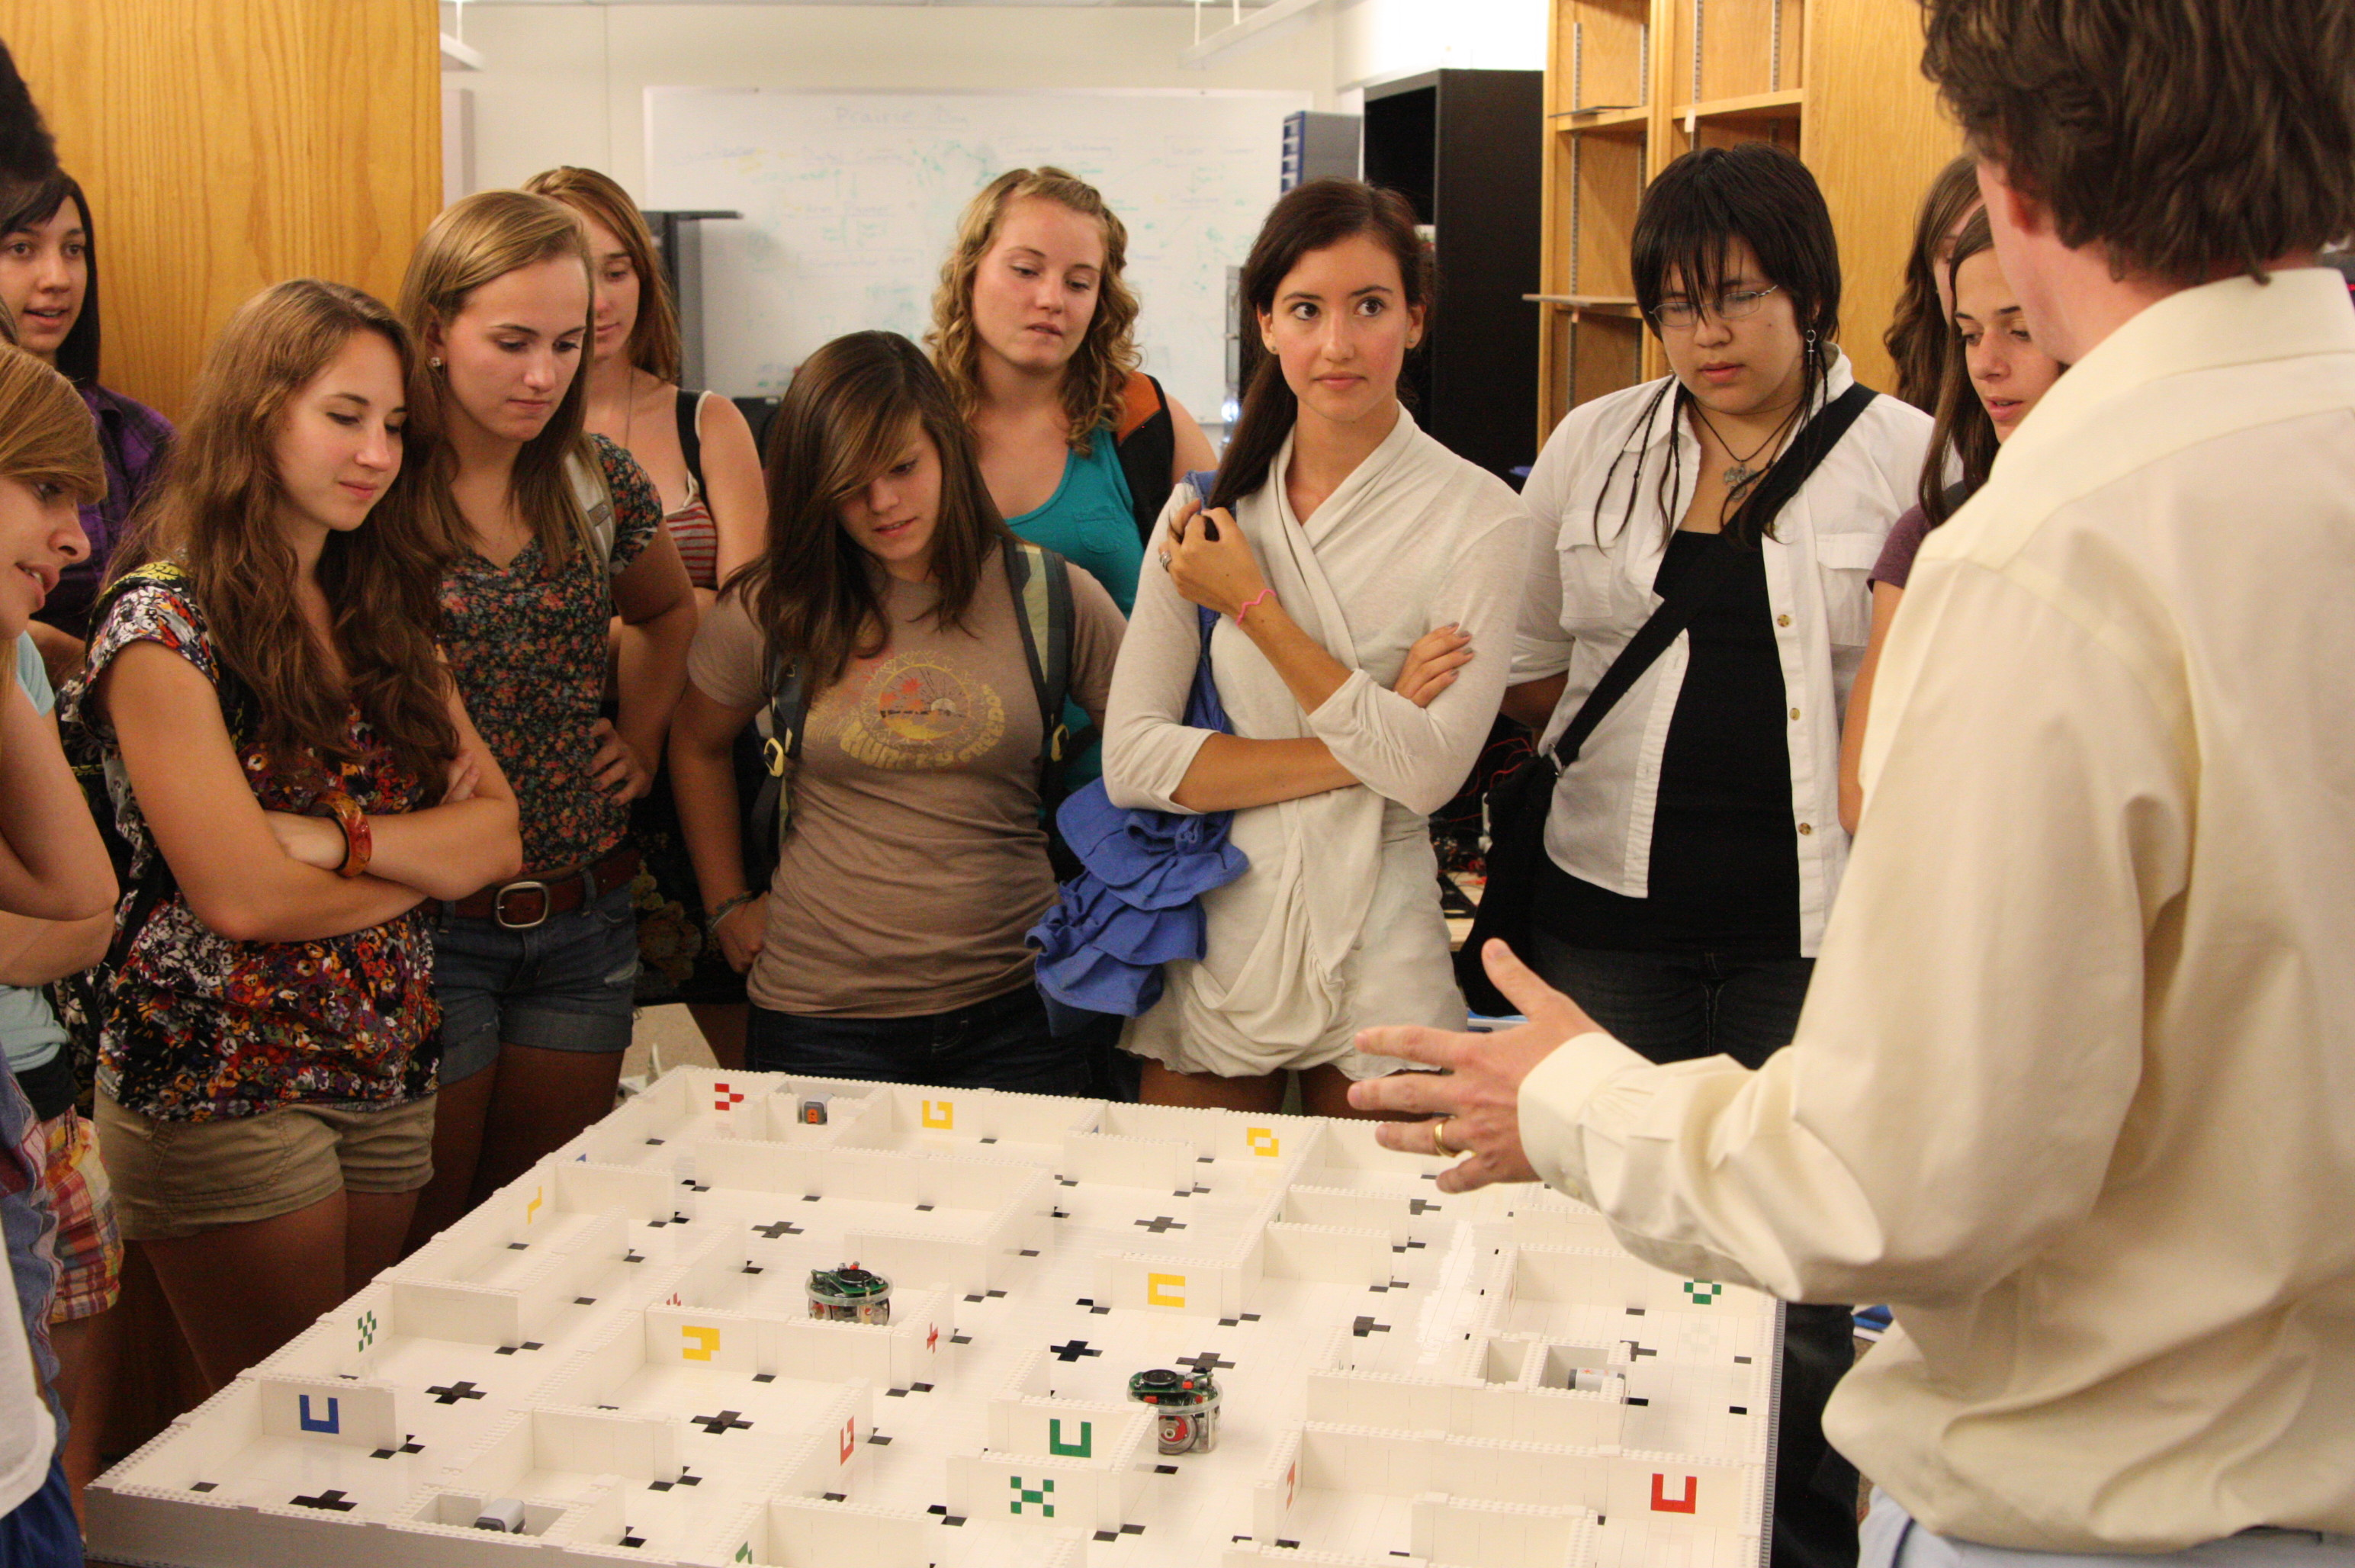
\includegraphics[width=0.48\textwidth]{figs/ratslife_real}
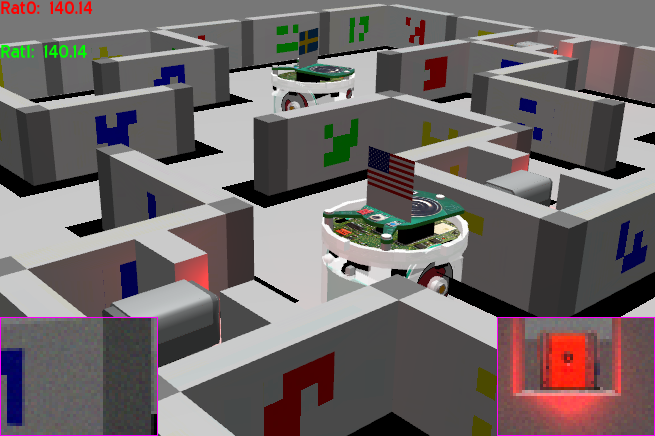
\includegraphics[width=0.48\textwidth]{figs/ratslife_webots}
\caption{由LEGO砖和e-Puck机器人(左)创建的“大屠杀”迷宫竞赛。在\emph{Webots}中模拟的相同环境。}
\label{fig:ratslifereal}
\end{figure}

% \subsection{Content}\label{sec:curr1content}
% After introducing the field and the curriculum using Chapter \ref{chap:introduction} ``\nameref{chap:introduction}'', another week can be spend on basic concepts from Chapter \ref{chap:locomotion} ``\nameref{chap:locomotion}'', which includes concepts like ``\nameref{sec:stability}'' and ``\nameref{sec:dof}''. The lab portions of the class can at this time be used to introduce the software and hardware used in the competition. For example, students can experiment with the programming environment of the real robot or setup a simple world in the simulator themselves.

% The lecture can then take up pace with Chapter \ref{chap:kinematics}. Here, the topics ``\nameref{sec:coordsystems}'', ``\nameref{sec:fwkmobile}'', and ``\nameref{sec:ivkmobile}'' are on the critical path, whereas other sections in Chapter \ref{chap:kinematics} are optional. It is worth mentioning that the forward kinematics of non-holonomic platforms, and in particular the motivation for considering their treatment in velocity rather than position space, are not straightforward and therefore at least some treatment of arm kinematics is recommended. These concepts can easily be turned into practical experience during the lab session. 

% The ability to implement point-to-point motions in configuration space thanks to knowledge of inverse kinematics, directly lends itself to ``\nameref{sec:maps}'' and ``\nameref{chap:pathplanning}'' treated in Chapter \ref{chap:pathplanning}. For the purpose of maze solving, simple algorithms like Dijkstra's and A* are sufficient, and sampling-based approaches can be skipped. Implementing a path-planning algorithm both in simulation and on the real robot will provide first-hand experience of uncertainty. 

\subsection{内容}
\label{sec:curr1content}
在引用该领域和课程后,使用Chapter\ref{chap:introduction}“\nameref{chap:introduction}”,可以从Chapter\ref{chap:locomotion}“\nameref{chap:locomotion}”,其中包括“\nameref{sec:stability}”和“\nameref{sec:dof}”等概念。课堂的实验室部分此时可以用来介绍比赛中使用的软件和硬件。例如,学生可以对真实机器人的编程环境进行实验,或者在模拟器中设置一个简单的世界。

然后,讲座可以跟上第\ref{chap:kinematics}的步伐。在这里,主题“\nameref{sec:coordsystems}”,“\nameref{sec:fwkmobile}”和“\nameref{sec:ivkmobile}”在关键路径上,而其他部分Chapter\ref{chap:kinematics}是可选的。值得一提的是,非完整平台的正向运动学,特别是考虑其在速度而不是位置空间处理的动机并不直接,因此至少有一些手臂运动学的处理被推荐。这些概念可以在实验室会议期间轻松转化为实际经验。

由于反向运动学的知识,在配置空间中实现点对点运动的能力直接适用于“\nameref{sec:maps}”和“\nameref{chap:pathplanning}”\ref{chap:pathplanning}。为了迷宫解决的目的,像Dijkstra和A*这样简单的算法就足够了,而且可以跳过基于抽样的方法。在模拟和真实机器人中实现路径规划算法将提供不确定性的第一手体验。

% The lecture can then proceed to ``\nameref{chap:sensors}'' (Chapter \ref{chap:sensors}), which should be used to motivate uncertainty using concepts like accuracy and precision. These concepts can be formalized using materials in Chapter \ref{chap:statistics} ``\nameref{chap:statistics}'', and quantified during lab. Here, having students record the histogram of sensor noise distributions is a valuable exercise. 

% Chapters \ref{chap:vision} and \ref{chap:feature_extraction}, which are on ``\nameref{chap:vision}'' and ``\nameref{chap:feature_extraction}'', do not need to extend further than needed to understand and implement simple algorithms for detecting the unique features in the maze environment. In practice, these can usually be detected using basic convolution-based filters from Chapter \ref{chap:vision}, and simple post-processing, introducing the notion of a ``feature'', but without reviewing more complex image feature detectors. The lab portion of the lab should be aimed at identifying markers in the environment, and can be scaffolded as much as necessary. 

% Indepth experimentation with sensors, including vision, serves as a foundation for a more formal treatment of uncertainty in Chapter \ref{chap:uncertainty} ``\nameref{chap:uncertainty}''. Depending on whether the ``\nameref{sec:linefitting}'' example has been treated in Chapter \ref{chap:feature_extraction}, it can be used here to demonstrate error propagation from sensor uncertainty, and should be simplified otherwise. In lab, students can actually measure the distribution of robot position over hundreds of individual trials (this is an exercise that can be done collectively if enough hardware is available), and verify their math using these observations. Alternatively, code to perform these experiments can be provided, giving the students more time to catching up. 

然后,讲座可以进入“\nameref{chap:sensors}”(Chapter\ref{chap:sensors}),这些概念应该用于通过精度和精度等概念来激发不确定性。这些概念可以使用章节\ref{chap:statistics}``\nameref{chap:statistics}'中的材料进行形式化,并在实验室量化。在这里,让学生记录传感器噪声分布的直方图是一项有价值的练习。

“\nameref{chap:vision}”和“\nameref{chap:feature_extraction}”的章节\ref{chap:vision}和\ref{chap:feature_extraction}不需要进一步扩展比理解和实现用于检测迷宫环境中的独特功能的简单算法所需要的。在实践中,通常可以使用Chapter\ref{chap:vision}中的基于卷积的滤波器和简单的后处理,引入“特征”的概念来检测这些滤波器,但不检查更复杂的图像特征检测器。实验室的实验室部分应该旨在识别环境中的标记物,并且可以根据需要进行脚手架化。

传感器(包括视觉)的深入实验,可作为更为正式的不确定性处理的基础,参见“第一章不确定性”,“不确定性”。根据\ref{chap:feature_extraction}中的“\nameref{sec:linefitting}”示例是否已被处理,可以在这里用于演示传感器不确定度的错误传播,否则应该简化。在实验室中,学生可以实际测量数百个单独测试中机器人位置的分布情况(如果有足够的硬件可用,这是一个可以集体完成的练习),并使用这些观察验证他们的数学。或者,可以提供执行这些实验的代码,使学生有更多的时间赶上。

% The localization problem introduced in Chapter \ref{chap:localization} is best introduced using Markov localization, from which more advanced concepts such as the particle filter and the Kalman filter can be derived. Performing these experiments in the lab is involved, and are best done in simulation, which allows neat ways to visualize the probability distributions changing. 

% The lecture can be concluded with ``\nameref{sec:ekfslam}'' in Chapter \ref{chap:slam}. Actually implementing EKF SLAM is beyond the scope of an undergraduate robotics class and is achieved only by very few students who go beyond the call of duty. Instead, students should be able to experience the workings of the algorithm in simulation, e.g., using one of the many available Matlab implementations, or scaffolded in the experimental platform by the instructor. 

% The lab portion of the class can be concluded by a competition in which student teams compete against each other. In practice, winning teams differentiate themselves by the most rigorous implementation, often using one of the less complex algorithms, e.g., wall following or simple exploration. Here, it is up to the instructor incentivizing a desired approach. 

% Depending on the pace of the class in lecture as well as the time that the instructor wishes to reserve for implementation of the final project, lectures can be offset by debates, as described in Section \ref{sec:debates}. 

Chapter\ref{chap:localization}中介绍的本地化问题最好使用马尔可夫定位,从中可以推导出更高级的概念,如粒子滤波器和卡尔曼滤波器。涉及实验中的这些实验,最好在模拟中进行,这样可以使整齐的方式可视化概率分布的变化。

讲座可以在\ref{chap:slam}的“\nameref{sec:ekfslam}”中得出结论。实际执行EKFSLAM超出了本科机器人课程的范围,只有极少数超越职责的学生才能实现。相反,学生应该能够在模拟中体验算法的运作,例如,使用许多可用的Matlab实现之一,或由教师在实验平台中构架。

课程的实验室部分可以由学生团队相互竞争的比赛结束。在实践中,获胜团队通过最严格的实施来区分自己,通常使用较不复杂的算法之一,例如墙跟踪或简单的探索。在这里,由教师鼓励想要的方法。

根据讲座课程的速度以及指导员希望为实施最终项目而预留的时间,演讲可以通过辩论来抵消,如第\ref{sec:debates}部分所述。

% \section{An introduction to autonomous manipulation}
% Although robotic manipulation is a much less mature field than autonomous mobile robots, teaching its basics, such as those treated in this book, is slightly easier, mainly due to the fact that concepts like uncertainty and non-holonomy are mostly absent. Robotic manipulation is also well suited for a practice-based curriculum due to the wide array of cheap, multi-DOF robotic arms. These, of course, quickly reach their limitations to demonstrate advanced topics such as dynamics or force control, which are beyond the scope of this book.

\section {自动操作介绍}
虽然机器人操纵是一个比自动移动机器人更不成熟的领域,但教授其基础知识(如本书中所讨论的那些)的基础知识稍微简单一些,主要是由于事实上不确定性和非整体性的概念大多缺席。机器人操纵也非常适合基于实践的课程,由于各种便宜的多自由度机器人手臂。这些当然可以很快地达到限制,以展示诸如动力学或力量控制等先进的主题,这超出了本书的范围。

% \subsection{Overview} 
% A manipulation-driven curriculum can be motivated by a ``grand challenge'' task such as robotic agriculture, robotic construction or assisted living, all of which have a manipulation problem at their core. Although a class project is likely to be limited to a toy-example, taking advantage of modern motion-planning frameworks and visualization tools, e.g. ROS/Moveit!, makes it easy to put the class into an industry-relevant framework and expose the students to state of the art platforms in simulation.

\subsection{概述}
以操纵为导向的课程可以通过“大挑战”的任务,如机器人农业,机器人建设或辅助生活等,其所有操作问题都是核心的。虽然课程项目可能仅限于玩具实例,但利用现代运动规划框架和可视化工具,例如,ROS/Moveit!,可以轻松将课堂放在行业相关的框架中,让学生们了解到模拟中最先进的平台。

% \subsection{Materials} 
% Possible class project range from ``robot gardening'' or ``robots building robots'', for which setups can easily be created. These include real or plastic cherry tomato or strawberry plants and robotic construction kits such as Modular Robotics ``Cubelets'', which easily snap together and have the advantage to form structures that are robots themselves, adding additional motivation. The robot arm, such as the open-source, 7-DOF CLAM arm, can be mounted on a portable structure that contains fixed a set of fixed (3D) cameras. In order to allow a large number of students to get familiar with the necessary software and hardware, the instructor can provide a virtual machine with a preinstalled Linux environment and simulation tools. In particular, using the ``Robot Operating Systems'' (ROS) allows recording so-called ``bag''-files of sensor values, including entire sequences of joint recordings and RGB-D video. This allows the students to work on a large part of the homeworks and project preparation from a computer lab or from home, maximizing availability of real hardware.

\subsection{材料}
可能的课程范围从“机器人园艺”或“机器人建筑机器人”,可以轻松地创建设置。这些包括真实的或塑料的樱桃番茄或草莓植物和机器人建筑工具包,如模块化机器人“Cubelets”,它们很容易地卡在一起,并具有形成机器人本身的结构的优势,增加了额外的动力。诸如开源7自由度CLAM臂的机器人手臂可以安装在包含固定的一组固定(3D)相机的便携式结构上。为了让大量学生熟悉必要的软​​件和硬件,教师可以为虚拟机提供预安装的Linux环境和仿真工具。特别地,使用“机器人操作系统”(ROS)可以记录传感器值的所谓“包”文件,包括联合记录和RGB-D视频的整个序列。这允许学生从计算机实验室或家中进行大部分的家庭作业和项目准备工作,从而最大限度地提高实际硬件的可用性。

% \subsection{Content}
% The first two weeks of this curriculum can be mostly identical to that described in Section \ref{sec:curr1content}. If a message passing system such as ROS is used, a good exercise is to record a histogram of message passing times in order to get familiar with the software.

% In Chapter \ref{chap:kinematics}, the focus is instead on manipulating arms, including the Denavit-Hartenberg scheme and numerical methods for inverse kinematics. In turn, the topics ``\nameref{sec:fwkmobile}'', and ``\nameref{sec:ivkmobile}'' do not necessarily need to be included. Forward and inverse kinematics can be easily turned into lab sessions using Matlab/Mathematica, simulation or a real robot platform. If the class uses a more complex or industrial robot arm, an alternative path is to record joint trajectories in a ROS bag and letting the students explore this data, e.g., sketching 

\subsection{内容}
本课程的前两周可以与\ref{sec:curr1content}部分中描述的大致相同。如果使用诸如ROS的消息传递系统,一个很好的练习是记录消息传递时间的直方图,以便熟悉该软件。

在\ref{chap:kinematics}中,重点是操纵手臂,包括Denavit-Hartenberg方案和逆运动学的数值方法。反过来,主题“\nameref{sec:fwkmobile}”和“\nameref{sec:ivkmobile}”不一定需要包括在内。使用Matlab/Mathematica,模拟或真正的机器人平台,可以轻松地将前向和反向运动学变为实验室。如果课程使用更复杂或工业的机器人手臂,另一种途径是在ROS包中记录关节轨迹,并让学生探索这些数据,例如素描

% \section{Class debates}\label{sec:debates}
% Class debates are a good way to decompress at the end of class and require the students to put the materials they learned in a broader context. Student teams prepare pro and contra arguments for a statement of current technical or societal concern, exercising presentation and research skills. Sample topics include \emph{Robots putting humans out of work is a risk that needs to be mitigated}; \emph{Robots should not have the capability to autonomously discharge weapons / drive around in cities (autonomous cars)}; or \emph{Robots need to be made from components other than links, joints, and gears in order to reach the agility of people}.

% The students are instructed to make as much use as possible of technical arguments that are grounded in the course materials and in additional literature. For example, students can use the inherent uncertainty of sensors to argue for or against enabling robots to use deadly weapons. Similarly, students relate the importance and impact of current developments in robotics to earlier inventions that led to industrialization, when considering the risk of robots putting humans out of work. 

% Although suspicious as first, students usually receive this format very well.  While there is agreement that debates help to prepare them for the engineering profession by improving presentation skills, preparing engineers to think about questions posed by society, and reflecting up-to-date topics, the debates seem to have little effect on changing the students' actual opinions on a topic. For example, in a questionnaire administered after class, only two students responded positively. Students are also undecided about whether the debates helped them to better understand the technical content of the class. Yet students find the debate concept important enough that they prefer it over a more in-depth treatment of the technical content of the class, and disagree that debates should be given less time in class. However, students are undecided whether debates are important enough to merit early inclusion in the curriculum or to be part of every class in engineering. 

% Concerning the overall format, students find that discussion time was too short when allotting 10 minutes per position and 15 minutes for discussion and rebuttal. Also, students tend to agree that debates are an opportunity to decompress (``relaxing''), which is desirable as this period of class coincides with wrapping up the course project.

\section{课堂辩论} 
\label{sec:debates}
课堂辩论是在课堂结束时解压缩的好方法,要求学生将他们学到的材料放在更广泛的背景下。学生团队就现有的技术或社会关切声明,演讲和研究技能准备专业和反驳论证。示例主题包括\emph{机器人让人失去工作是一种需要缓解的风险};\emph{机器人不应该有能力在城市(自治汽车)自主地排放武器/驱动器};或\emph{机器人需要由链接,关节和齿轮以外的组件制成,以达到人们的敏捷性}。

指导学生尽可能多地利用基于课程材料和其他文献的技术论据。例如,学生可以使用传感器固有的不确定性来争论机器人使用致命的武器。同样,当考虑机器人使人失去工作的风险时,学生将当前机器人技术发展的重要性和影响与导致工业化的早期发明联系起来。

虽然可疑是第一,学生通常收到这种格式很好。虽然协议有助于通过提高演讲技巧为工程专业做好准备,准备工程师考虑社会提出的问题,反映最新的话题,但辩论似乎对改变学生的“一个话题的实际意见。例如,在上课后进行的问卷调查中,只有两名学生积极回应。这些辩论是否有助于他们更好地了解课堂的技术内容,学生们也不确定。然而,学生发现辩论理念足够重要,他们更喜欢更深入地对待课堂的技术内容,不同意辩论的时间应该更少。不过,无论辩论是否足够重要,学生都不能确定,以便早日纳入课程或成为每一个工程类课程的一部分。

关于整体格式,学生发现,讨论时间太短,每位10分钟,15分钟的讨论和反驳。此外,学生倾向于同意辩论是减压的机会(“放松”),这是可取的,因为这个课堂时期与课程项目的结束一致。